\documentclass{article}
\usepackage{microtype}
\usepackage{graphicx}
\usepackage{booktabs}
\usepackage{hyperref}
\newcommand{\theHalgorithm}{\arabic{algorithm}}
\usepackage{icml2026}
\usepackage{amsmath,amssymb,amsthm,mathtools}
\usepackage{longtable}
\newtheorem{theorem}{Theorem}
\newtheorem{proposition}[theorem]{Proposition}
\newtheorem{corollary}[theorem]{Corollary}
\newcommand{\E}{\mathbb{E}}
\newcommand{\Var}{\operatorname{Var}}
\newcommand{\Cov}{\operatorname{Cov}}
\newcommand{\ind}{\mathbf{1}}
\newcommand{\PPI}{\text{PPI}}
\input{artifacts/tables/macros.tex}
\icmltitlerunning{Fixed-Score Confidence Intervals: Conditional Gains and Finite-Sample Costs}
\begin{document}
\twocolumn[
\icmltitle{Fixed-Score Confidence Intervals:\\Conditional Gains and Finite-Sample Costs}
\begin{icmlauthorlist}
\icmlauthor{Anonymous Author}{anon}
\end{icmlauthorlist}
\icmlaffiliation{anon}{Anonymous Institution}
\icmlkeywords{prediction-powered inference, confidence intervals, control variates}
\vskip 0.3in
]
\printAffiliationsAndNotice{}
\begin{abstract}
Can confidence intervals become narrower when labels, unlabeled observations, and a supplied predictor cannot change? For binary population means, we separate nonlinear information in an immutable score from the cost of exploiting it with valid inference. A control-variate decomposition characterizes the oracle variance improvement beyond affine PPI++, while pilot-conditioned binary component intervals provide finite-sample coverage without retraining the base predictor. In a prespecified low-disagreement synthetic setting, the latter intervals reduce mean width by \ExactGain\% (paired 95\% Monte Carlo interval: \ExactGainLo--\ExactGainHi\%) against full-budget exact label-only intervals. The gain disappears with a smaller unlabeled pool, higher disagreement, and two real empirical populations; a larger \NonlinearGain\% Wald reduction instead exhibits undercoverage. These are conditional-gain and negative-result findings, not a new general PPI principle, an exhaustive literature comparison, or a claim of universally shorter valid intervals.
\end{abstract}

\section{Introduction}
Expensive gold-standard measurements and plentiful model scores arise in remote sensing, astronomy, and scientific model evaluation. Prediction-powered inference (PPI) uses a labeled residual correction to turn these scores into valid inference rather than accepting their predictions as truth \citep{angelopoulos2023ppi}. The practical question here is narrower than improving the predictor: after both datasets and their predictions have been collected, can a different inferential use of exactly those inputs produce a shorter confidence interval?

Three distinctions determine the answer. First, PPI++ already optimizes the affine correction to a supplied score \citep{angelopoulos2024ppiplus}; comparing only with untuned PPI overstates remaining room. Second, low variance and valid coverage are different objectives. A narrow plug-in normal interval need not achieve its nominal level at a scientifically relevant sample size. Third, our guarantee is over repeated sampling, not conditional coverage given all realized labeled and unlabeled inputs. We keep inputs identical \emph{across methods within a repetition}, and assess unconditional repeated-sampling coverage under an explicit model.

We study binary prevalence, $\theta=\E Y$, because it directly represents quantities such as the proportion of deforested plots or galaxies with spiral arms. Binary labels also permit exact finite-sample probability inversion, so the strict coverage question need not be answered by a normal approximation alone. We only use functions of the immutable score $Z=f(X)$ as inference controls. This permits fitting a small correction using existing labels but never changes $f$, adds a label, or enlarges the unlabeled sample. If immutability were instead interpreted as forbidding even fitted inference controls, only prespecified score maps would be admissible; that is a stricter problem.

Our contribution is an evidence-backed \emph{conditional-gain analysis}. A variance identity isolates the conditional-mean information not represented by an affine score. Nested finite-dimensional controls test this headroom without weakening the PPI++ baseline. A pilot-conditioned, signed composition of three exact binomial intervals then tests whether a gain survives finite-sample coverage requirements. The resulting tradeoff is concrete: low disagreement and a sufficiently large existing unlabeled pool can help, whereas affine conditional means, conservative uncertainty composition, and rare labels can eliminate an apparent improvement. On the supplied real-data empirical populations, additional gains beyond affine PPI++ are small, and the exact construction is wider than label-only exact inference.

These methods use standard control-variate projection and PPI rectification ideas. No algorithmic priority claim is made. The study deliberately restricts its literature access to directly supplied starter papers and an older concentration reference, under an independent-research access constraint. Thus neither absence of other related work nor novelty over the full literature is established. This limitation is material to evaluating the contribution.

\section{Setting and Related Work}
\label{sec:setting}
We observe independent iid samples
\[
 L=\{(Y_i,Z_i)\}_{i=1}^n,\qquad U=\{\widetilde Z_j\}_{j=1}^N,
\]
with the same score marginal, $Y\in\{0,1\}$ and $Z\in[0,1]$. The supplied predictor is fixed externally; equivalently, condition on an independently trained predictor while preserving this sampling model. Sample sizes, transformations, and folds are prespecified. Our target is a superpopulation mean, not an unknown mean of a finite pool sampled without replacement. Known score bounds are an assumption, not the empirical extrema of one sample.

\paragraph{PPI and PPI++.}
For a fixed score function $h$, the mean estimator is
\begin{equation}
 T_h=\overline{Y-h(Z)}_L+\overline{h(Z)}_U.
 \label{eq:est}
\end{equation}
Original PPI sets $h(z)=z$; its residual correction removes fixed prediction bias \citep{angelopoulos2023ppi}. PPI++ uses $h(z)=\lambda z$. Its oracle coefficient is
\begin{equation}
 \lambda_* = \frac{\Cov(Y,Z)}{(1+n/N)\Var(Z)},
 \label{eq:lambda}
\end{equation}
not the infinite-$N$ coefficient. We reproduce the published mean plug-in convention: labeled covariance and prediction variance pooled over $L\cup U$, with an unconstrained real coefficient \citep[Example 6.1]{angelopoulos2024ppiplus}. Negative coefficients are allowed, especially for anticorrelated scores. Affine score rescaling alone cannot improve this oracle. PPI/PPI++ normal intervals are asymptotic; original PPI also gives finite-sample component-composition constructions.

\paragraph{Different resource freedoms.}
StratPPI studies designed within-stratum sampling with fixed known weights and positive limiting allocations \citep{fisch2024strat}. Those assumptions do not automatically hold after splitting an already-collected iid labeled set into score bins. We therefore do not report a mis-specified known-weight stratified interval as a valid comparator. Our series controls retain the uncertainty of finite unlabeled scores. Cross-PPI trains or fine-tunes fold-specific predictors on the same labels \citep{zrnic2024cross}; using fixed-score control fits here does not invoke its predictor-stability theorem. Active inference designs which observations receive labels \citep{zrnic2024active}. Neither model training nor prospective label allocation is available in this task.

\paragraph{Nonasymptotic composition.}
The finite-sample intervals below specialize the original PPI union-bound rectification recipe, rather than introducing that principle anew. For bounded residuals we use the empirical-Bernstein (EB) inequality of \citet[Theorem 4]{maurer2009}. For binary indicators we use binomial-tail inversion (Clopper--Pearson, CP), with its elementary coverage argument in Appendix~\ref{app:proofs}. Both yield conservative finite-sample intervals; being valid does not make either shortest.

\section{What Information Remains in a Fixed Score?}
\label{sec:theory}
Let $m(z)=\E[Y\mid Z=z]$, $a=N/(n+N)$, and let $\Pi_{\mathrm{aff}}m$ denote the $L^2$ projection of $m(Z)$ onto $\operatorname{span}\{1,Z\}$. All controls below have finite second moments. Additive constants in $h$ cancel in~\eqref{eq:est}.

\begin{theorem}[Score-only oracle headroom]
\label{th:oracle}
For a fixed control independent of the inference samples, let $C=1/n+1/N$. Then
\begin{align}
 V(h)&=\Var(T_h)=\frac{\Var(Y-h)}{n}+\frac{\Var(h)}{N},\\
 &=\frac{\Var(Y)-a\Var(m)}{n}+C\Var(h-am).
 \label{eq:complete}
\end{align}
Thus $h_*=am+c$ minimizes variance over all score-measurable controls. If $\Var(Z)>0$, the affine-oracle excess variance is
\begin{equation}
 V_{\mathrm{aff}}-V_{\mathrm{all}}
 =\frac an\E[(m-\Pi_{\mathrm{aff}}m)^2].
 \label{eq:gap}
\end{equation}
It vanishes exactly when $m$ is affine almost surely.
\end{theorem}
\begin{proof}
Unbiasedness and the first identity follow from matching marginals and sample independence. Since $\Cov(Y,h)=\Cov(m,h)$ and $a(1/n+1/N)=1/n$, completing the centered square gives~\eqref{eq:complete}. Least-squares orthogonality gives~\eqref{eq:gap}. Appendix~\ref{app:proofs} handles the remaining degeneracies.
\end{proof}

The minimal variance also equals
\begin{equation}
 V_{\mathrm{all}}=\frac{\E\Var(Y\mid Z)}n+
                     \frac{\Var(m)}{n+N}.
 \label{eq:oraclevar}
\end{equation}
An existing score cannot eliminate unexplained label variation. A binary score admits only affine score functions on its support, hence no nonlinear headroom. A constant score offers no score-only gain. Conversely, zero correlation with the original score need not imply no information: a symmetric U-shaped conditional mean can have nonzero $\Var(m)$ and zero $\Cov(Y,Z)$.

The oracle width ratio to affine PPI++ is the square root of the corresponding variance ratio, for nondegenerate normal first-order intervals. It is \emph{not} a theorem of finite-sample interval dominance. Nor is~\eqref{eq:gap} a lower bound for every conceivable procedure using additional features, parametric assumptions, or a different sampling design.

\subsection{Nested fitted controls and asymptotic inference}
Partition $[0,1]$ into $B$ fixed equal-width bins and take
\[
 \phi_B(z)=(z,\ind\{b(z)=0\},\ldots,\ind\{b(z)=B-2\}).
\]
With $G=\Cov(\phi_B)$ positive definite and $c=\Cov(\phi_B,Y)$, the optimal coefficient is $\beta_*=aG^{-1}c$. Series$B$ estimates $c$ from labels and $G$ from all observed scores, using ridge $10^{-3}/n$. This class contains the raw affine score; histogram-only controls do not. A fixed basis may fail to capture some nonlinear information even when~\eqref{eq:gap} is positive.

For fixed $B$, bounded features, a fixed law with positive limiting variance, and $n/N\to r\in(0,\infty)$, the coefficient fit is consistent. The estimation remainder is exactly
\begin{equation}
 (\widehat\beta-\beta_*)^\top
 (\overline\phi_U-\overline\phi_L)=o_P(n^{-1/2}).
 \label{eq:rem}
\end{equation}
A two-sample CLT and consistent residual/pooled-feature variances therefore justify asymptotic Wald inference. This argument does not assume independence of a fitted coefficient and the observations that fit it. Singular population feature covariances, increasing dimensions, or selecting the narrowest observed interval are outside this theorem.

We additionally evaluate four-bin histogram plug-in (Hist4), balanced five-fold cross-fitted histograms (CFHist4), and oracle $am(Z)$ on synthetic data only. Each histogram uses two pseudo-observations at its training-label mean per bin. Cross-fitting changes only the control fit, not $f$. Its justification is a fixed-fold first-order expansion, not independent-fold finite-sample variance; Appendix~\ref{app:proofs} supplies that argument.

\section{Finite-Sample Coverage Without New Inputs}
\label{sec:exact}
Use the first $p=\lfloor n/5\rfloor$ labeled observations as a fixed pilot and the remaining $m=n-p$ as inference labels. The pilot is part of the original budget. Conditional on its full labeled pairs, a pilot-fitted control is fixed, and the remaining observations still satisfy the iid model. All compared learned-control procedures share this split. Stronger full-budget label-only and fixed-map baselines are retained.

\subsection{Bounded-control empirical Bernstein}
For an iid sample $x$ of size $t\ge2$ in a known interval of span $R$, define
\begin{equation}
 e(x,R,\delta)=\sqrt{\frac{2s_x^2\log(4/\delta)}t}
 +\frac{7R\log(4/\delta)}{3(t-1)},
 \label{eq:eb}
\end{equation}
where $s_x^2$ uses denominator $t-1$. Two applications of the one-sided EB inequality give error at most $\delta$ \citep{maurer2009}. Fit any pilot-measurable $g\in[0,1]$ and let $h=a_mg$, $a_m=N/(N+m)$. Residuals have known span $1+a_m$; unlabeled controls have span $a_m$. Adding their radii at $\delta=\alpha/2$ gives a finite-sample $1-\alpha$ interval centered at~\eqref{eq:est}, then intersected with $[0,1]$. Each radius uses $\log(8/\alpha)$. The empirical sample range cannot replace these known spans.

We compare raw-score, clipped pilot-linear, and pilot-histogram EB controls, plus full-budget and same-split label-only EB. Larger residual range, label splitting, and the union bound can consume a real variance gain. No empirical-Bernstein dominance is asserted.

\subsection{Binary signed-component intervals}
Choose a binary map $b(Z)$ using only the pilot. Our learned map thresholds the four smoothed bin means at $1/2$. The identity
\begin{equation}
 \theta=q+p_+-p_-,\quad
 \begin{cases}
 q=\Pr(b(Z)=1),\\
 p_+=\Pr(Y=1,b(Z)=0),\\
 p_-=\Pr(Y=0,b(Z)=1)
 \end{cases}
 \label{eq:binary}
\end{equation}
holds regardless of the map's accuracy. Estimate $q$ on all $N$ unlabeled scores and $p_+,p_-$ on the $m$ remaining labeled pairs. Use a two-sided CP interval of error $\alpha/3$ for each binomial count. For their endpoints, return
\begin{equation}
 C_{\mathrm{bin}}=[\ell_q+\ell_+-u_-,\ u_q+u_+-\ell_-]\cap[0,1].
 \label{eq:compose}
\end{equation}
We call this interval CPRectHist, a binary PPI composition with a learned inference map.

\begin{proposition}[Pilot-conditional coverage]
\label{prop:finite}
Under the model in Section~\ref{sec:setting}, a pilot-measurable binary map, $m,N\ge1$, and fixed $0<\alpha<1$, interval~\eqref{eq:compose} covers $\theta$ with probability at least $1-\alpha$ conditional on the pilot, and hence unconditionally.
\end{proposition}
\begin{proof}
Given the pilot, each of the three counts is marginally binomial with its stated probability. CP inversion bounds its miss probability by $\alpha/3$. A union bound covers all components; signed interval arithmetic and~\eqref{eq:binary} yield the claim. The two error counts need not be independent.
\end{proof}

The fixed raw map $b(z)=\ind\{z\ge1/2\}$ requires no pilot, so CPRectRawFull uses \emph{all} labels. We also retain a same-split raw version and full-budget label-only CP. CPRectHist may be much wider than these competitors. Its exact mathematical guarantee does not certify every floating-point beta quantile by interval arithmetic; numerical edge and binomial-grid tests accompany the implementation.

\subsection{When can the composition be shorter?}
A transparent diagnostic is a symmetric score partition with $q=1/2$ and disagreement probability $\epsilon$, so $p_+=p_-=\epsilon/2$. Let $m/n\to c$ and $N/n\to\kappa$. Once the pilot learns the correct binary partition, the leading-order CP-width ratio to label-only CP is
\begin{equation}
 \frac{z_{1-\alpha/6}}{z_{1-\alpha/2}}
 \frac{\sqrt{1/(4\kappa)}+
 2\sqrt{(\epsilon/2)(1-\epsilon/2)/c}}{1/2}.
 \label{eq:cplimit}
\end{equation}
This is a binomial-normal-inversion width diagnostic, not a finite-$n$ coverage approximation for~\eqref{eq:compose}, whose coverage is already exact. It shows both low disagreement and a sufficiently large \emph{existing} unlabeled pool are important. For $\kappa=1$, this particular conservative composition has no leading-order advantage even at zero disagreement. A different exact interval might improve on this construction; no impossibility claim for all exact procedures follows.

\section{Experiments}
\label{sec:experiments}
\subsection{Protocol, datasets, and comparisons}
All methods receive identical labeled values, scores, and unlabeled scores in each repetition. No model training, prospective allocation, additional labeling, or sample enlargement occurs within a comparison. Varying $n,N$ across experiments is a sensitivity analysis, not an additional resource given to one method. All nominal intervals use $\alpha=.05$. Intersecting with $[0,1]$ preserves coverage; an empty intersection is retained as empty, with zero width and no coverage.

\paragraph{Known-truth synthetic laws.}
Except for the explicitly invalid shift stress test, $Z,\widetilde Z$ are iid uniform on $[0,1]$, and $Y\mid Z\sim\mathrm{Bernoulli}(m(Z))$. Central laws are linear $m=.1+.8Z$, anticorrelated $m=.9-.8Z$, uninformative $m=.5$, U-shaped $m=.05+.9\ind\{Z<.25\text{ or }Z\ge.75\}$, and rare $m=.002+.04\ind\{Z\ge.9\}$. Their means are $.5$ except rare, whose mean is $.006$. A separately prespecified finite-sample supplement uses sharp U-shaped $m=.005+.99\ind\{Z<.25\text{ or }Z\ge.75\}$. The shape and error probabilities are frozen generators, not fitted using hidden unlabeled labels. Oracle controls use the known formula only as explicitly infeasible diagnostics.

\paragraph{Real empirical populations.}
We use galaxies and forest from the pinned \texttt{ppi-python==0.2.3} example data: respectively 16,743 and 1,596 paired labels/precomputed scores. Both label arrays are binary; no missing values occur, and scores lie in $[0,1]$. The empirical means are approximately $.259273$ and $.151629$. Forest has only 252 distinct scores; duplicated score values are retained, not mistaken for iid sampling violations. We independently sample labeled and unlabeled indices \emph{with replacement} from each fixed empirical distribution. Methods never receive labels at sampled unlabeled indices. Coverage targets that known empirical-law mean; it does not establish iid sampling, gold-standard quality, or external scientific validity of the original data collection. Raw-data licensing is not separately specified by the pinned package; download provenance and hashes are provided, without claiming its MIT code license covers data.

\paragraph{Repetitions and chronology.}
The main suite has 10,000 repetitions per central synthetic law at $n=1000,N=10000$; 3,000 per sample-size, finite-ratio, and real-data setting; and 20,000 for rare $n=200,N=2000$. Independent ablations have 3,000 per law. The finite-sample supplement has 5,000--10,000 per setting. Totals are 103,000 main, 12,000 ablation, and 65,000 supplementary repetitions; deterministic reruns are not extra evidence. Small pilot runs tested execution/runtime only. The binary supplement was motivated by EB's concentration cost and preregistered before its own results were examined; its chronology is distinct from the original primary experiment. No confirmatory configuration was tuned to gain or coverage afterward.

\paragraph{Uncertainty and validity assessment.}
We report Wilson 95\% Monte Carlo (MC) intervals for marginal coverage and paired delta-method 95\% MC intervals for ratios of mean widths. Ratios are not averages of within-repetition ratios. Four prespecified nonlinear Series/PPI++ contrasts and four sharp CPRectHist/label-CP contrasts form separate Holm-corrected width-test families. Coverage intervals and other comparisons are descriptive, not simultaneous. All four tests in the first family and three in the second support smaller mean width after correction; the $N=n$ sharp setting is wider. Width significance does not rescue undercoverage. In particular, a coverage MC interval containing $.95$ is not proof of exact validity, and all covered repetitions do not prove coverage one.

\begin{table*}[t]
\caption{Full-budget asymptotic comparison at $n=1000,N=10000$. Series4/PPI++ is the paired ratio of mean widths, with 95\% MC intervals. Coverage brackets are marginal Wilson 95\% MC intervals, not guarantees or multiplicity-adjusted tests. Narrower normal intervals do not count as finite-sample-valid gains.}
\label{tab:asym}
\centering\small
\input{artifacts/tables/asymptotic.tex}
\end{table*}

\subsection{Nonlinear headroom does not certify finite-sample validity}
Table~\ref{tab:asym} and Figure~\ref{fig:main} separate the large synthetic opportunity from modest empirical gains. In the U-shaped law, raw-score covariance is zero, so oracle affine PPI++ cannot exploit the conditional mean. Series4 reduces mean width by \NonlinearGain\% and approaches the score-function oracle, as the projection calculation predicts. Yet its coverage is $94.43\%$, with MC interval $[93.96,94.86]\%$, below the nominal target. PPI++ itself is $94.53\%$ in this setting. CFHist4 has $94.71\%$ coverage, with MC interval $[94.25,95.13]\%$; that is not a finite-sample certificate either. These are asymptotic-efficiency evidence and finite-sample warnings, not a strict-validity success.

Linear and anticorrelated laws have no additional nonlinear oracle headroom. Their tiny Series width decreases therefore cannot be interpreted as new information; fitting and variance estimation can slightly narrow intervals at the cost of calibration. A histogram-only class can even lose the original score's linear signal. Galaxies and forest reductions are only \GalaxyGain\% and \ForestGain\%, respectively. Thus strong simulation gains should not be extrapolated to substantial real-data improvement beyond affine PPI++.

Small-label empirical calibration is worse. At $n=200,N=10000$, Series4 coverage is $92.73\%$ on galaxies (Wilson interval $[91.75,93.61]\%$) and $91.40\%$ on forest ($[90.34,92.35]\%$). PPI++ itself covers $93.90\%$ and $93.40\%$, respectively. Series4 mean biases are approximately $-.00479$ and $-.00615$. These observed finite-sample biases are warnings, not a proved sole explanation of undercoverage; small apparent width gains are not usable as strict-validity improvements.

\begin{figure*}[t]
\centering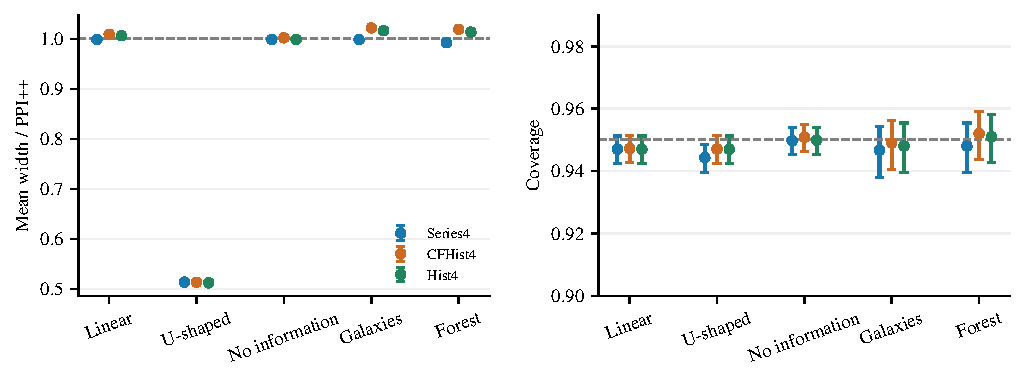
\includegraphics[width=.95\textwidth]{figures/main.pdf}
\caption{Asymptotic-control comparisons on the same main-suite inputs, $n=1000,N=10000$. Left: paired mean-width ratios to PPI++ (95\% MC bars). Right: coverage with marginal Wilson 95\% MC bars. The nonlinear gain is substantial, but the normal intervals have no finite-sample guarantee. Linear/no-information settings serve as negative controls.}
\label{fig:main}
\end{figure*}

\subsection{Finite-sample gains are conditional and smaller}
Table~\ref{tab:exact} and Figure~\ref{fig:exact} use only the separate binary supplement. In the low-disagreement sharp law at $n=1000,N=10000$, CPRectHist has mean width $.04455$, versus $.06287$ for full-budget label-only CP: a reduction of \ExactGain\% (95\% MC interval \ExactGainLo--\ExactGainHi\%). All 10,000 CPRectHist repetitions covered; the Wilson lower endpoint is $99.96\%$, while the theorem supplies the distribution-wide $95\%$ guarantee under its hypotheses. The observed overcoverage is substantial conservatism, not exact nominal calibration.

The same construction is only $13.90\%$ narrower at $n=200,N=2000$, and $32.28\%$ narrower at $n=4000,N=40000$. With $n=N=1000$ it is $54.37\%$ \emph{wider}. With the moderate U-shaped disagreement level, it is wider than label-only CP despite the large normal-oracle headroom. It is also wider on both real empirical laws. Raw-threshold exact PPI composition, even using all labels, cannot exploit the sharp U shape; its failure shows the value of the map, not a new general rectification principle. This is an aligned-bin positive control: its boundaries coincide with the prespecified four-bin grid. It does not demonstrate a learning-specific advantage over a suitable prespecified nonlinear map; a DGP-informed fixed map would avoid the pilot's inference-label cost, but is not generally available without knowing the relationship.

EB makes the conservatism particularly visible. In the sharp $n=1000,N=10000$ setting, EBHist4 mean width is $.10731$, well above label-only CP and CPRectHist. In the moderate U-shaped main setting, EBHist4 is $.13533$, whereas full-label EB is $.11409$. Pilot isolation and boundedness retain validity but do not guarantee a net width gain. These failed routes remain in the report rather than being replaced by whichever interval looked shortest on the inference data.

\begin{table*}[t]
\caption{Finite-sample-valid binary composition versus full-budget label-only exact CP, in the separate supplementary suite. Both have mathematical coverage at least $95\%$ under the iid model. Width-ratio brackets are paired 95\% MC intervals; coverage brackets are marginal Wilson intervals. Sharp settings use 5,000 repetitions except $(1000,10000)$, which uses 10,000; other rows use 5,000.}
\label{tab:exact}
\centering\small
{\setlength{\tabcolsep}{4pt}\input{artifacts/tables/exact.tex}}
\end{table*}

\begin{figure*}[t]
\centering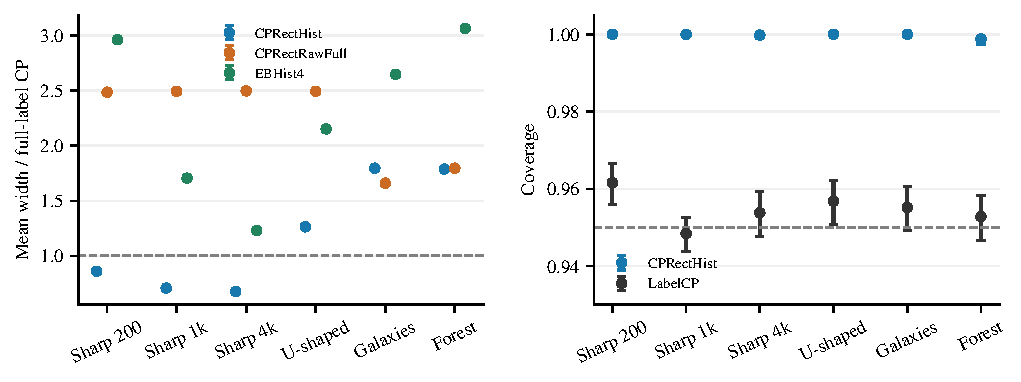
\includegraphics[width=.95\textwidth]{figures/exact.pdf}
\caption{Exact-coverage methods, same inputs per supplementary repetition. Left: paired mean-width ratios to full-label CP, with 95\% MC bars. Right: CPRectHist and label-CP coverage with Wilson bars. Exact guarantees coexist with substantial overcoverage; gains occur in the low-disagreement synthetic condition, not the real empirical laws. EBHist4 is also valid but much wider.}
\label{fig:exact}
\end{figure*}

\subsection{Ablations and failure mechanisms}
\paragraph{Nested basis, bins, and fitting.}
We fix $B=4$ before confirmation and ablate $B\in\{1,2,4,8,16\}$ on independent repetitions, never selecting the best observed interval. Series1 is affine-only; adding indicators retains the affine class. In the U-shaped law, two bins do not encode the symmetric extremes, whereas four aligned bins do. Beyond four, further bin splitting supplies no additional conditional-mean signal and can increase estimation cost. On the linear law, histogram-only binning discards within-bin signal, whereas the nested series retains it. Full results include real-data ablations and a same-label histogram fit, so cross-fitting is not credited with creating nonlinear information. Figure~\ref{fig:ablation} presents the main mechanism; sample-size/oracle sensitivity is in Appendix~\ref{app:protocol}.

\paragraph{Rare outcomes defeat fitted Wald intervals.}
For iid Bernoulli mean $p>0$, all labeled outcomes are zero with probability $(1-p)^n$. Label Wald, zero-covariance PPI++, and the tested mean-fitted controls then return $[0,0]$. Their coverage is at most $1-(1-p)^n$. At $p=.006,n=200$ the analytic ceiling is $69.99\%$, and PPI++ achieves only \RareCoverage\%. More unlabeled scores do not change that event. Exact CP and EB avoid zero-width collapse. Appendix Table~\ref{tab:safety} reports coverage and widths; even the synthetic oracle normal interval need not be reliable with rare labels.

\paragraph{Mismatched score populations invalidate rectification.}
In the shift stress test, labeled scores remain uniform, but unlabeled scores are $\mathrm{Beta}(2,5)$; the target remains the labeled-law mean. Matching marginals fails, so score-mean differences are not mean-zero. Series4 has zero observed coverage; many support intersections become empty, yielding near-zero mean width. This is an invalidity signal, not an efficiency gain. Label-only CP remains applicable. Apparent EB robustness in one shift setting does not extend its theorem beyond matching populations.

\begin{figure*}[t]
\centering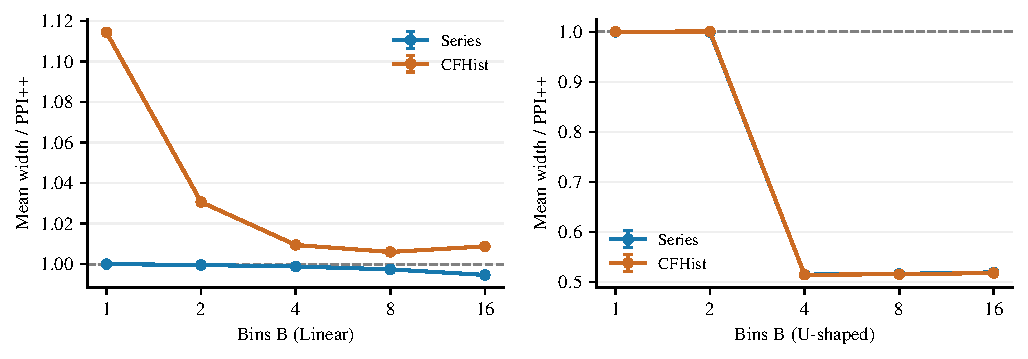
\includegraphics[width=.95\textwidth]{figures/ablation.pdf}
\caption{Independent bin-count ablations ($3,000$ repetitions per law, $n=1000,N=10000$). Lines connect paired ratios of mean width to PPI++; bars are 95\% MC intervals. Series includes the raw-score feature, CFHist does not. More bins are not automatically better; the fixed four-bin design captures the prespecified U shape. All curves are asymptotic methods, not exact coverage guarantees.}
\label{fig:ablation}
\end{figure*}

\section{Discussion, Limitations, and Conclusion}
\label{sec:discussion}
\paragraph{Answer to the fixed-input question.}
There can be shorter valid intervals without more labels or a different base predictor. The gain comes from a better use of existing score information, not a resource change. In this study a theorem-backed binary composition is narrower in a low-disagreement nonlinear setting, but finite-sample protection costs much of the normal-oracle advantage. There is no universal shortening: affine conditional means have zero nonlinear score-only oracle headroom, a finite basis may miss nonlinear structure, and even informative scores may not offset splitting and uncertainty-composition penalties. These no-gain statements have different scopes and should not be conflated with a minimax impossibility theorem.

\paragraph{Practical implications.}
Prespecify the inference control and guarantee class before inspecting the remaining labels or interval widths. Compare against tuned, unconstrained finite-ratio PPI++, not merely raw PPI, and against full-budget exact label-only inference when strict binary coverage matters. A strong coverage theorem does not imply near-nominal tightness; a small MC width error bar does not imply statistical validity. When labels are rare, the all-zero event provides a simple analytic warning before optimizing coefficients.

\paragraph{Limitations.}
This is a restricted independent study of binary means and score-only controls. It does not establish novelty relative to unsearched literature, global optimality, or superiority to every available exact PPI construction. The positive exact result uses a deliberately favorable low-error synthetic mechanism. Real-data analyses are resampling experiments on supplied empirical laws, not new remote-sensing or astronomy conclusions; the original predictor-training independence and annotation provenance were not independently established. Known-weight designed stratification, additional features, finite-population corrections, quantiles, regression parameters, growing control classes, and distribution shift require separate analysis. Numerical CP inversion is tested in ordinary floating-point arithmetic, not formally verified rounding. Conservative CP composition can be improved in principle, but post-hoc choosing the shortest reported interval would require selection-safe coverage not supplied here.

\paragraph{Conclusion.}
The defensible answer is conditional: nonlinear score information provides variance headroom, but valid finite-sample shortening additionally requires that fitting and coverage costs be affordable. Our exact positive result, real-data near-null findings, and normal-interval failures delimit those conditions rather than promise a universally narrower confidence interval.

\section*{Impact Statement}
This work examines the statistical use of existing predictions and does not collect new human labels or train a new predictor. Undercoverage in rare-event or shifted populations can mislead scientific decisions; the intended benefit is explicit separation of validity from apparent precision. The empirical-law benchmarks do not justify scientific or policy decisions about the original populations. Source data may inherit annotation errors or sampling bias, and their independent licensing is not established by a package's code license. The manuscript and reproducibility artifacts were prepared with an AI research assistant; mathematical audits and deterministic reruns reduce, but do not eliminate, the need for human scientific review.

\bibliography{references}
\bibliographystyle{icml2026}

\clearpage
\onecolumn
\appendix
\section{Complete Proofs and Assumption Audit}
\label{app:proofs}
\subsection{Oracle projection and no-gain statements}
For $h$ independent of the two inference samples, matching score marginals imply $\E T_h=\E Y$. Sample independence implies the displayed $V(h)$. Center $h$ and $m$ without loss of generality. The conditional-expectation identity yields $\Cov(Y,h)=\Cov(m,h)$. With $C=1/n+1/N$ and $Ca=1/n$,
\[
 V(h)=\frac{\Var(Y)}n-\frac{2\Cov(m,h)}n+C\Var(h)
 =\frac{\Var(Y)-a\Var(m)}n+C\Var(h-am).
\]
The final variance is nonnegative and zero exactly when $h-am$ is constant almost surely. For $\Var(Z)>0$, projecting $m$ onto $1,Z$ explains $\Cov(m,Z)^2/\Var(Z)=\Cov(Y,Z)^2/\Var(Z)$. Pythagoras gives Theorem~\ref{th:oracle}. Total variance gives~\eqref{eq:oraclevar}. If $\Var(Z)=0$, every measurable function of $Z$ is constant almost surely, so no score-mean difference can help. On support with two distinct score values, any function is affine on that support. If $m$ is constant, all score functions have zero covariance with $Y$ and cannot improve the fixed-control oracle over labels alone. These are control-class statements; no claim of uniformly shortest confidence intervals follows.

For any nested fixed feature class $\mathcal H$ containing constants and the raw score, the same argument yields
\[
 V_{\mathcal H}-V_{\mathrm{all}}=(a/n)\E[(m-\Pi_{\mathcal H}m)^2].
\]
Consequently its oracle variance cannot exceed the affine oracle. This does not say every nonlinear $m$ is represented by our chosen four-bin basis, nor that estimated variances preserve finite-sample ordering. For example, if $m(Z)=Z$ with uniform $Z$, histogram-only controls lose within-bin information. With $B$ equal-width bins, their oracle variance is larger than affine by $a/(12nB^2)$. The nested Series$B$ class avoids this approximation disadvantage.

\subsection{Vector plug-in studentization}
Assume a fixed distribution; independent matching samples; deterministic $n,N\to\infty$ with $n/N\to r\in(0,\infty)$; prespecified fixed-dimensional bounded features; positive-definite $G$; and positive limiting root-$n$ variance. The labeled cross-covariance and pooled feature covariance converge to $c,G$. Since ridge $\rho_n=10^{-3}/n\to0$, $\widehat\beta=a_n(\widehat G+\rho_n I)^{-1}\widehat c$ differs from $\beta_{*,n}=a_nG^{-1}c$ by $o_P(1)$. The finite-ratio $a_n$ need not equal its limit at every $n$. Bounded feature second moments imply $\Delta_\phi=\overline\phi_U-\overline\phi_L=O_P(n^{-1/2})$, proving~\eqref{eq:rem} without a fitted-coefficient independence assumption.

An ordinary two-sample CLT for the deterministic limiting coefficient gives
\[
 \sqrt n(T_{\widehat\beta}-\theta)\ \Rightarrow\
 N(0,\sigma^2),\quad
 \sigma^2=\Var(Y-\beta_*^\top\phi)+r\beta_*^\top G\beta_*.
\]
The implemented variance is
\[
 \widehat V=s_L^2(Y-\widehat\beta^\top\phi)/n+
                   \widehat\beta^\top\widehat G\widehat\beta/N.
\]
Expanding sample residual variance into bounded labeled moments shows $n\widehat V\to_P\sigma^2$. Slutsky gives nominal asymptotic coverage. For binary $Y$ with $0<\theta<1$ and $r>0$, the oracle variance is positive; degeneracies are not automatically covered by a nondegenerate normal theorem. The numerical ridge permits a sample solve but does not by itself establish a theorem for singular population covariances or distributions changing with $n$. For the studied real arrays, each score bin has positive empirical mass and within-bin score variation; no nonzero affine-plus-indicator combination is constant on that support.

The histogram plug-in uses smoothed bin heights, not this ridge coefficient formula. Nevertheless, fixed positive bin probabilities imply each smoothed height converges to its bin conditional mean; finitely many bins imply uniform height convergence. The same finite-vector mean-difference and moment arguments justify its asymptotic Wald interval. Neither fitted rule is exactly unbiased at finite $n$.

\subsection{Cross-fitted histogram expansion}
Take fixed $B$, fixed $K\ge2$, positive bin masses, balanced data-independent folds, and the same ratio/nondegeneracy conditions. Every fold has at least two inference observations for its sample variance. For fold $k$, fit $h_k$ on the full labeled pairs outside that fold. Two pseudo-observations per bin vanish relative to its growing counts. Thus, for deterministic $h_{0,n}=a_n\E[Y\mid b(Z)]$, $\|h_k-h_{0,n}\|_\infty\to_P0$ over the finite bins.

Condition on the entire complement-training sigma field, not only its outcomes. For $e_k=h_k-h_{0,n}$ and balanced sizes $n_k=n/K,N_k=N/K$, the held-out difference has mean zero and conditional variance
\[
 \Var(\overline e_{U_k}-\overline e_{L_k}\mid\mathcal F_{-k})
 =(1/n_k+1/N_k)\Var_Z(e_k(Z))
 \le (1/n_k+1/N_k)\E_Z[e_k(Z)^2].
\]
After multiplication by $n$, the bound converges to zero in probability. Conditional Chebyshev, integrating its bound truncated at one, implies the difference is $o_P(n^{-1/2})$. Fixed $K$ permits summing these remainders even though training sets overlap. The resulting first-order estimator is the full-sample fixed-histogram oracle. The code's foldwise variance
\[
 \widehat V_{\rm CF}=K^{-2}\sum_{k=1}^K
 [s_{L_k}^2(Y-h_k)/n_k+s_{U_k}^2(h_k)/N_k]
\]
converges to that oracle variance at the required scale by boundedness and foldwise LLNs. It is not an exact variance formula for mutually independent fitted folds. No growing-$K$, growing-bin, arbitrary flexible-fit, or observation-sorted-fold claim is made.

\subsection{Empirical-Bernstein guarantee}
\citet[Theorem 4]{maurer2009} states a one-sided bound for iid $[0,1]$ variables with $\sqrt{2s^2\log(2/\eta)/t}+7\log(2/\eta)/(3(t-1))$. Its pairwise-difference variance equals ordinary unbiased sample variance because $\sum_{i<j}(x_i-x_j)^2=t\sum_i(x_i-\bar x)^2$. Apply the theorem to $W=(x-A)/R$ and $1-W$, each at $\eta=\delta/2$, to obtain~\eqref{eq:eb}. Scaling is already incorporated in $s_x^2$; only the additive term needs the explicit span factor.

Conditional on the pilot, $h=a_mg\in[0,a_m]$, so $Y-h\in[-a_m,1]$. Both inference sample sizes must be at least two. Use error $\alpha/2$ for each component and union bound; matching score marginals make their expectations sum to $\theta$. Independence of the two coverage events is unnecessary. Integrating conditional coverage gives unconditional coverage. The pilot-linear fit uses at least two pilot observations; all experiment configurations satisfy this. Label-only EB has span one and uses all $n$ labels with $\delta=\alpha$.

\subsection{Clopper--Pearson and binary signed composition}
For integer count $K=k$ in $t\ge1$ Bernoulli trials and error $\eta$, CP endpoints are
\[
 \ell(k)=\begin{cases}0,&k=0,\\F^{-1}_{\mathrm{Beta}(k,t-k+1)}(\eta/2),&k>0,\end{cases}\quad
 u(k)=\begin{cases}1,&k=t,\\F^{-1}_{\mathrm{Beta}(k+1,t-k)}(1-\eta/2),&k<t.\end{cases}
\]
The lower endpoint solves $\Pr_{\ell(k)}(K\ge k)=\eta/2$; the upper solves $\Pr_{u(k)}(K\le k)=\eta/2$. Binomial-tail monotonicity bounds each directional miss by $\eta/2$, including boundary endpoints. Thus total error is at most $\eta$; discreteness can yield larger coverage.

For fixed binary $b$, the pointwise identity
$Y=b(Z)+\ind\{Y=1,b(Z)=0\}-\ind\{Y=0,b(Z)=1\}$ gives~\eqref{eq:binary}. Conditional on an independent pilot, the learned map is fixed and each component count remains binomial. Set $\eta=\alpha/3$, union bound the three valid marginal intervals, and use the negative sign to reverse the last interval endpoints. Their joint event implies~\eqref{eq:compose}. The positive/negative counts are not independent, and independence is not used. A raw fixed map needs no pilot, so its stronger full-label comparator is feasible under exactly the same budget. Selecting the shortest of several such intervals from inference-data widths is \emph{not} justified by these marginal guarantees.

The leading-order diagnostic~\eqref{eq:cplimit} uses interior binomial probabilities and normal inversion, for which each component CP length is $2z_{1-\alpha/6}\sqrt{p(1-p)/t}+o_P(t^{-1/2})$. Adding the three lengths and dividing by label-only $2z_{1-\alpha/2}\sqrt{\theta(1-\theta)/n}$ gives the expression. In the symmetric fixed-bin laws, pilot means converge to $\epsilon$ or $1-\epsilon$, so for $0<\epsilon<1/2$ the learned partition equals the true partition with probability tending to one. This diagnostic is not a uniform finite-sample width theorem or a guarantee under changing rare-event probabilities. At the boundary $\epsilon=0$, the two zero-error CP lengths are $O(m^{-1})$ rather than the interior normal order, while the $q=1/2$ length is $O(N^{-1/2})$. Thus for $N=n$ the limiting ratio is still $z_{1-\alpha/6}/z_{1-\alpha/2}>1$, justifying the zero-disagreement statement separately.

\subsection{Rare-event obstruction}
If all $n$ labels are zero, labeled means/covariances vanish. Scalar PPI++ then has coefficient zero; the nested series has a zero cross-covariance vector; smoothed histograms and every complement-training histogram have zero global and bin means. The named fitted normal intervals all equal $[0,0]$. For Bernoulli $p>0$, that event has probability $(1-p)^n$, yielding coverage at most $1-(1-p)^n$. This includes the exact-zero coefficient rule and does not depend on $N$. It is not a bound for all inference procedures: raw-score residual controls, a known oracle map, EB additive terms, and exact binomial inversion need not collapse. For fixed $p$, the obstruction vanishes asymptotically, so it does not contradict a pointwise CLT.

\section{Detailed Protocol, Provenance, and Reproducibility}
\label{app:protocol}
\subsection{Frozen settings and randomness}
The root seed is 20261103. NumPy SeedSequence namespaces are $[20261103,1]$ for execution pilots, $[20261103,2]$ for main, $[20261103,3]$ for ablations, and $[20261103,4]$ for the exact supplement. Child streams follow the frozen configuration-list order; manifests save entropy, spawn keys, repetition counts, runtimes, file hashes, and sample sizes. Every method shares all arrays and folds within a repetition. Label draws use only labeled scores. The synthetic unlabeled generator never draws outcome labels. On empirical laws the simulator uses the full label array only to define truth and draw labeled examples; no sampled unlabeled labels are passed to inference functions. Duplicate indices across independent with-replacement draws do not violate the empirical-law observation model, although they do not represent additional scientific units.

The main suite includes all five central synthetic laws at $(n,N)=(1000,10000)$; linear and U-shaped sensitivity at $(200,2000),(4000,40000),(1000,1000)$; both real laws at $n\in\{200,1000\},N=10000$; rare $(200,2000)$; and shift $(1000,10000)$. Ablations independently run linear, U-shaped, galaxies, and forest at $(1000,10000)$. Exact-supplement sharp settings are $(200,2000),(1000,10000),(4000,40000),(1000,1000)$; moderate U, linear, no-information, rare, galaxies, and forest use $(1000,10000)$, plus rare $(200,2000)$.

The pilot is the first fifth of iid unsorted labeled pairs. Five cross-fitting folds are contiguous index blocks in both arrays; iid order makes those assignments data-independent. Histogram bin edges are fixed at multiples of $1/B$, with the right endpoint included in the final bin. Empty training bins get the global training mean through the two-pseudo-observation rule. Series$B$ uses the score plus $B-1$ bin indicators and a vanishing ridge; raw PPI++ does not clip its coefficient. Normal critical values, coverage error, pseudo-counts, bins, ridge, and split fraction are not tuned on confirmatory results.

\subsection{Monte Carlo calculations}
Let $W_{ir}$ be method $i$'s width in repetition $r$, $\bar W_b$ a paired baseline mean, and $\widehat R=\bar W_i/\bar W_b$. Its estimated MC standard error is
\[
 \widehat{\mathrm{se}}(\widehat R)=\frac{s(W_i-\widehat R W_b)}{\bar W_b\sqrt{R_{\mathrm{rep}}}}.
\]
Normal $\widehat R\pm1.96\widehat{\mathrm{se}}$ intervals report simulation uncertainty in the mean ratio, not interval-width spread or uncertainty of one scientific dataset. Width mean SE is $s(W_i)/\sqrt{R_{\mathrm{rep}}}$. Coverage uses Wilson binomial intervals. Bias and RMSE are included in the machine-readable summary. Empty parameter-space intersections have zero width and no coverage; they are never discarded or relabeled as successful short intervals.

One-sided paired width-difference tests use their Monte Carlo normal approximation. Holm adjustment is applied separately to the four original nonlinear Series4/PPI++ settings and four sharp CPRectHist/full-CP settings. Extremely small tail probabilities can underflow to zero numerically; those outputs mean below floating-point resolution, not mathematical probability zero. No coverage hypothesis-testing family or simultaneous coverage assessment is claimed. The primary inferential conclusions rely on the stated theorems and transparent empirical coverages, not on treating a nonsignificant coverage test as success.

\subsection{Data and access provenance}
Data files are downloaded through the two direct Google Drive identifiers in the datasets loader of the pinned 0.2.3 wheel. Wheel code was inspected only for that allowlisted loader, with no repository browsing, recommendations, discovery, or citation chasing. The full SHA-256 hashes, sizes, exact URLs, score duplicate fractions, and EDA checks are in \texttt{artifacts/data\_provenance.json}. Labels and scores are unaltered. Forest score duplicates are expected quantization/duplicates, not removed. No further dataset or deep model was trained.

Only the five directly supplied PPI-related papers and the 2009 EB reference were retrieved for methodological reading. Actual-read sections and exact versions are recorded in \texttt{literature/allowed\_methods.md}, \texttt{scope\_notes.md}, and the access ledger. No open literature search or attempt to identify the excluded prior work was made. No suspected forbidden encounter was recorded. Reference lists inside permitted papers were not pursued. Failed attempts to obtain NeurIPS 2026 style URLs returned 404; the official ICML 2026 archive was obtained directly from \url{https://media.icml.cc/Conferences/ICML2026/Styles/icml2026.zip}. The official style file is unmodified; this manuscript uses the anonymous initial-submission layout, with its eight-page main-text cap. The Impact Statement follows the template guidance; ICML does not use the NeurIPS paper checklist. An additional filled reproducibility checklist is supplied below.

\subsection{Implementation audit and commands}
Implementation is scalar CPU NumPy/SciPy; no GPU or paid API is used. The environment is Python 3.11.15, NumPy 2.4.6, SciPy 1.17.1, pandas 3.0.6, and Matplotlib 3.11.2, with complete pins in \texttt{requirements.txt} and \texttt{requirements.lock}. BLAS/OpenMP threads are fixed to one for deterministic execution. Initial main, ablation, and exact runs took approximately 277, 76, and 109 seconds respectively on this host; final centered-code main and ablation replays took approximately 236 and 69 seconds. These are measured wall times with thread control, not a hardware-independent runtime guarantee. Dataset download, document reading, analysis, compilation, and audit time are separate.

Independent math audits found a fixed absolute variance cutoff that could disable PPI++ on tiny rescaled scores and incomplete input contracts. The cutoff was removed, scale invariance was regression-tested, and public complete evaluators now reject nonbinary, nonfinite, misaligned, and too-short inputs as appropriate. Exact binary helpers also reject broadcasting shapes. A subsequent paper review found raw-moment cancellation near nonzero score offsets. Common-anchor and centered within-/between-group variance arithmetic repaired it; high-precision independent checks and offset-plus-small-scale regression tests confirmed the repair. Series also anchors its score coordinate, without claiming ridge affine invariance. These were correctness repairs, not gain-seeking tuning. The early branch-repair replay had 21 SHA-identical main/ablation CSVs. After final centering, all 115,000 main/ablation repetitions were regenerated: the maximum endpoint/center/width change was $1.69\times10^{-13}$ and every coverage flag was unchanged. All 11 exact-suite CSVs were separately replayed with identical hashes. Final analysis uses the regenerated centered outputs, while both historical stages remain available. The final 16 tests cover coefficient formulas, constant scores, empty bins, bin endpoints, frozen arrays, scale/offset behavior, CP endpoints, exact binomial-grid coverage, signed components, and invalid inputs. Audit histories are retained rather than overwritten.

To reproduce from a fresh directory, install the pinned requirements, run \texttt{python code/fetch\_data.py}, then \texttt{python -m pytest -q tests}; run \texttt{python code/run\_experiments.py --mode main}, \texttt{--mode ablation}, and \texttt{python code/run\_exact.py}. Set \texttt{OPENBLAS\_NUM\_THREADS=1}, \texttt{OMP\_NUM\_THREADS=1}, and \texttt{MKL\_NUM\_THREADS=1}. Scripts refuse to overwrite existing raw results. From included outputs, \texttt{python code/analyze.py} regenerates every numerical table, plotted figure, and measured prose macro. \texttt{latexmk -pdf paper.tex} builds the PDF. \texttt{README.md} gives fresh-output-directory options and exact commands.

\begin{figure}[h]
\centering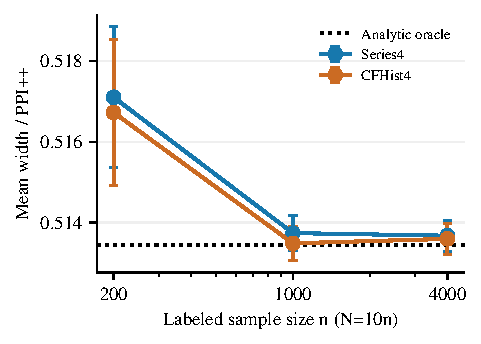
\includegraphics[width=.55\textwidth]{figures/sensitivity.pdf}
\caption{Prespecified nonlinear sample-size sensitivity at $N=10n$. Ratios use the same main inputs as PPI++; error bars are paired 95\% MC intervals. The dotted line is the analytic fixed-score oracle ratio from Theorem~\ref{th:oracle}, not an empirical result or a finite-sample coverage claim.}
\label{fig:sensitivity}
\end{figure}

\begin{table}[h]
\caption{Rare outcomes ($n=200,N=2000$, 20,000 repetitions) and the intentionally invalid shift condition ($n=1000,N=10000$, 3,000 repetitions). Matching marginals fail under shift; no PPI-based validity claim applies there. Near-zero width for Series4 under shift mainly reflects empty support intersections.}
\label{tab:safety}
\centering\small\input{artifacts/tables/safety.tex}
\end{table}

\subsection{Filled reproducibility and claim checklist}
\begin{itemize}
\item \textbf{Target and sampling stated: Yes.} Binary mean, independent matching samples, fixed predictor, empirical-law versus external-population distinction (Sections~\ref{sec:setting}, \ref{sec:experiments}).
\item \textbf{Finite-sample and asymptotic claims separated: Yes.} Exact CP and EB guarantees versus fixed-law Wald CLTs (Sections~\ref{sec:theory}, \ref{sec:exact}).
\item \textbf{All mathematical assumptions and proofs included: Yes within stated scope.} Singular features, rare events, growing classes, and mismatch limits are explicit (Appendix~\ref{app:proofs}). No minimax or uniform-width claim.
\item \textbf{Seeds, budgets, and hyperparameters fixed: Yes.} Protocol/amendment/supplement files and frozen configuration lists preserve chronology.
\item \textbf{Repeated results and uncertainty: Yes.} Raw repetition rows, Wilson coverage intervals, paired width uncertainty, and separate Holm families; no MC pass/fail masquerading as proof.
\item \textbf{Fair baselines: Yes within restricted scope.} Unconstrained finite-ratio PPI++, full-label CP/EB, same-split controls, full-label fixed binary-map exact comparator, nested affine-plus-bin control, and explicitly infeasible synthetic oracle.
\item \textbf{Failures and negative findings retained: Yes.} EB cost, weak real gains, small-unlabeled-pool loss, rare-label undercoverage, mismatch stress, and historical audit defects are documented.
\item \textbf{Every table/figure reproducible: Yes.} All generated by \texttt{code/analyze.py} from raw CSVs; appendix tables below include width MC SEs. Generated macros prevent manually invented prose values.
\item \textbf{Data/model provenance and licensing: Partly established.} Pinned example data, hashes and fixed scores supplied; external label/model validity and independent data licensing remain unverified. No independent data license is invented.
\item \textbf{Compute and environment: Yes.} CPU only, thread controls, dependencies, measured times, manifests, and commands included.
\item \textbf{Complete novelty/related-work survey: No.} Intentional access constraints preclude it. No priority or exhaustive superiority claim is made.
\item \textbf{Human subjects/new annotation: Not applicable.} No new data collection or labeling; inherited biases and errors remain possible.
\item \textbf{Numerical machine certification: No.} Mathematical exactness is distinct from tested floating-point CP implementation; no formal rounding proof is claimed.
\end{itemize}

\section{Complete Measured Comparison Tables}
All tables below are emitted from the supplied raw repetition files by \texttt{code/analyze.py}. Width intervals can be reconstructed from mean $\pm1.96$ MC SE; coverage intervals are marginal Wilson intervals. No rows are chosen by shortest observed width. The machine-readable \texttt{summary.csv} also contains bias and RMSE; \texttt{paired\_ratios.csv} contains every recorded paired comparison. Supplementary-suite estimates are not paired across suites with main-suite estimates.
\small
\input{artifacts/tables/full_main.tex}
\input{artifacts/tables/full_exact.tex}
\input{artifacts/tables/full_ablation.tex}
\end{document}
